% 闭合电流在匀强磁场中所受的力矩

%未完成
\pentry{安培力\upref{FAmp},力矩\upref{Torque}}
\begin{figure}[h]
\centering
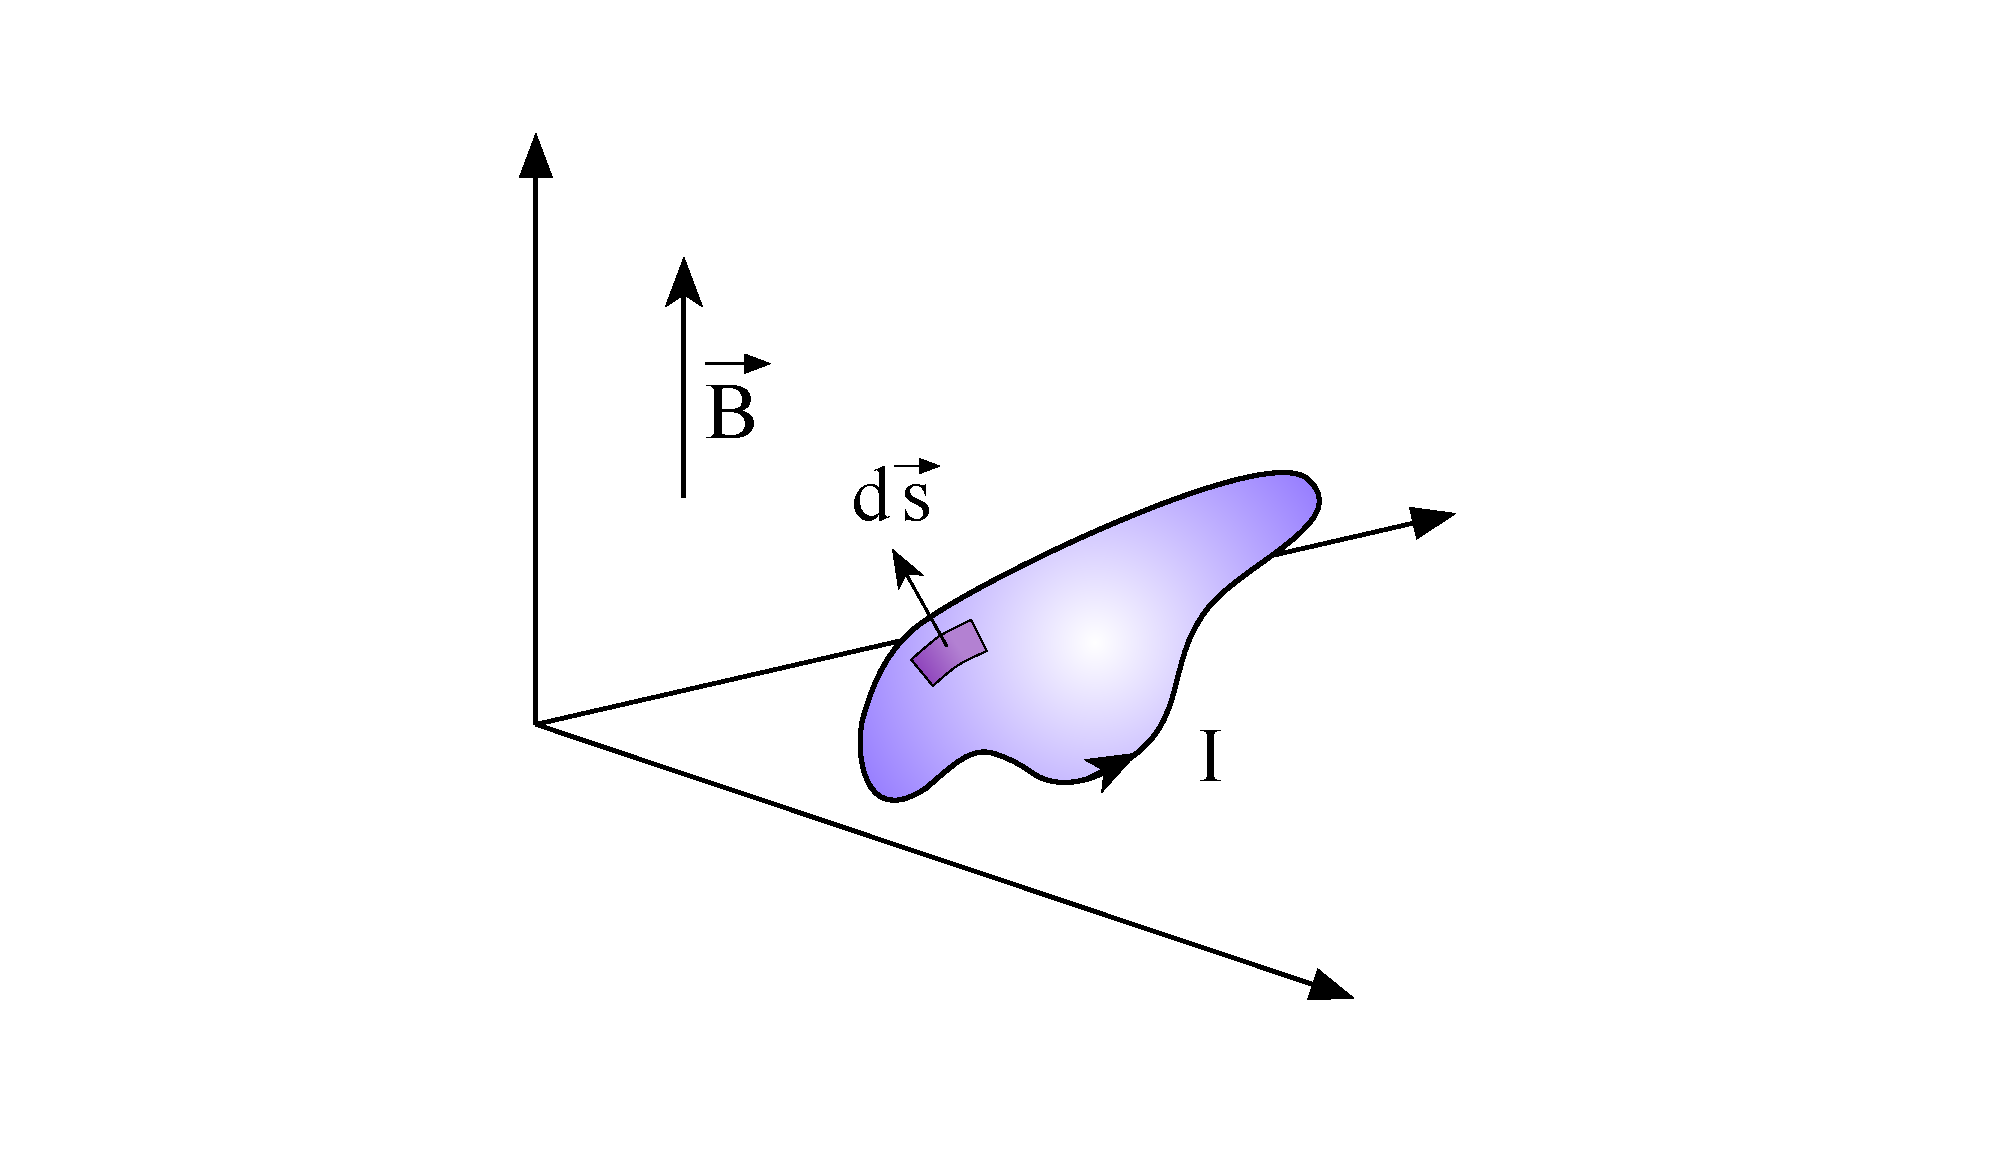
\includegraphics[width=10cm]{./figures/EBTorq.pdf}
\caption{闭合电流在磁场中所受的力矩} \label{EBTorq_fig1}
\end{figure}
如\autoref{EBTorq_fig1}, 线圈中有闭合电流 $I$, 以及任意磁场分布 $\vec B(\vec r)$, 现在求线圈所受力矩.我们可以把线圈划分为许多小段 $\D\vec r$,每小段的安培力产生的力矩为
\begin{equation}
\D\vec M = \vec r\cross \D F = \vec r \cross (I \D \vec r \cross \vec B)
\end{equation}
对连续叉乘进行化简\upref{TriCro} 得
\begin{equation}
\begin{aligned}
\D\vec M &=  {\vec r \cross \left( {I\D\vec r \cross \vec B} \right)} =  {I \left( {\vec B \vdot \vec r} \right)} \D\vec r  -  I{\vec B \left( {\vec r \vdot \D\vec r} \right)}
\end{aligned}
\end{equation}
对 $\vec r$ 沿闭合回路进行环积分得总力矩为
\begin{equation}
\begin{aligned}
\vec M & = \int \D\vec M = I\oint {\left( {\vec B\vdot\vec r} \right)\D\vec r}  - I\vec B\oint {\vec r \vdot \D\vec r }
\end{aligned}
\end{equation}
其中
\begin{equation}
\oint {\vec r \vdot \D\vec r}  = \oint {r \uvec r \vdot \D\vec r}  = \oint {r \D r}  = \left.\frac{r^2}{2}\right |_{r_0}^{r_0}  = 0 % 未完成: 这个符号有介绍吗?
\end{equation}
这是因为换积分的起点和终点到原点的距离都相同. 所以
\begin{equation}
\begin{aligned}
\vec M &= I\oint {\left( {\vec B \vdot \vec r} \right)\D\vec r} \\
&= \uvec x I \oint {\left( {\vec B \vdot \vec r} \right)\uvec x \vdot \D\vec r}  + \uvec y I \oint {\left( {\vec B \vdot \vec r} \right)\uvec y \vdot \D\vec r}  + \uvec zI \oint {\left( {\vec B \vdot \vec r} \right)\uvec z \vdot \D\vec r} 
\end{aligned}
\end{equation} 
对第一项进行分析,剩下两项类推即可
由斯托克斯定理得
\begin{equation}
\begin{aligned} 
\uvec x I \oint (\vec B \vdot \vec r)\uvec x \vdot \D\vec r  &= \uvec x I \int \curl [ ( \vec B \vdot \vec r)\uvec x] \vdot \D\vec s \\
&= \uvec x I \int \grad (\vec B \vdot \vec r) \cross \uvec x \vdot \D\vec s \\
&= \uvec x I \int \D\vec s  \cross \grad (\vec B \vdot \vec r) \vdot \uvec x 
\end{aligned} 
\end{equation}
其中面积分在以环路为边界的任意曲面进行.对 $\uvec y$ 和 $\uvec z$ 项也同样处理,得
\begin{equation}
\vec M = I \int \D\vec s\cross\grad(\vec B\vdot\vec r)
\end{equation}
这是最一般的力矩表达式.

当磁场为匀强磁场时,由于 $\grad \left( {\vec B \vdot \vec r} \right) = \vec B$
\begin{equation}
\vec M = I\left( {\int {\D\vec s} } \right) \cross \vec B
\end{equation}







